% ==========================================
% DESIGN AND IMPLEMENTATION
% ==========================================

\newpage
\chapter{THIẾT KẾ VÀ XÂY DỰNG}

\begin{concept}[15cm]
\textit{Nội dung chương này sẽ trình bày về các công việc đã thực hiện trong luận văn dựa trên những kiến thức nền được giới thiệu ở chương 2. Cụ thể, chương này sẽ tập trung giới thiệu việc kết hợp giữa hệ thống BE-PUM và công cụ NuSMV trong việc nhận dạng packer. Để có thể so sánh giữa phương pháp pháp nhận dạng packer thông qua chữ ký và phương pháp model checking, giải thuật nhận dạng packer thông qua chữ ký cũng được hiện thực và giới thiệu cụ thể trong chương này.}
\end{concept}

\section{Phát triển hệ thống BE-PUM để xử lý các packer}

\hspace{0.5cm}Để xử lý 14 kỹ thuật của packer. Hệ thống BE-PUM được hiện thực và giả lập môi trường thực thi bao gồm bộ nhớ và các thanh ghi:
\begin{itemize}
\item{\textbf{PEB và TIB}: Process Environment Block (PEB) dùng để lưu trữ các thông tin của Process và Thread Information Block (TIB) dùng để lưu trữ các thông tin của Thread hiện hành. Hình \ref {fig:TIBPEBArchi} mô tả lớp TIB và PEB được hiện thực trong hệ thống BE-PUM. Theo đó mỗi lần thực thi một câu lệnh tác động vào địa chỉ TIB của chương trình thì TIB và PEB sẽ được cập nhật tương ứng.
\begin{figure}
\centering
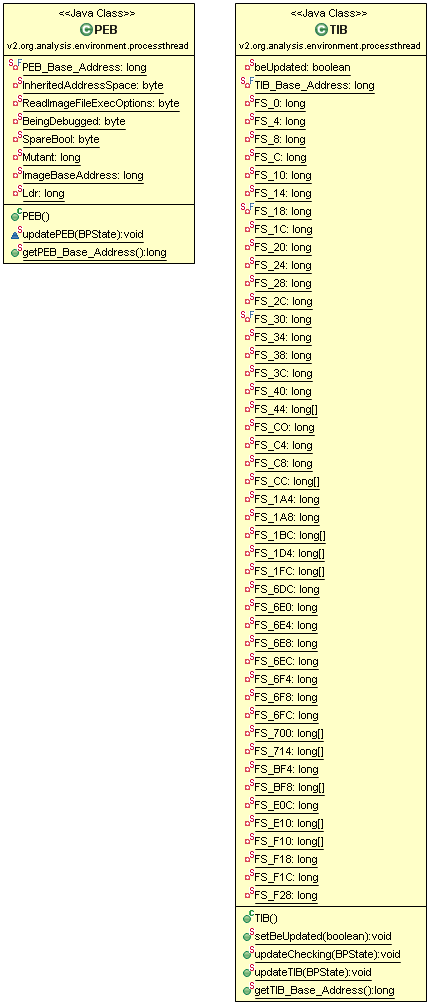
\includegraphics[width=0.5\textwidth]{tib_peb}
\caption{Cấu trúc của TIB và PEB}
\label{fig:TIBPEBArchi}
\end{figure}
}
\item{\textbf{LDR Data}: Loader Data được giả lập để có thể lưu trữ các thông tin của các thư viện liên kết động được nạp vào trong quá trình thực thi để gọi các API. Hình \ref {fig:LDRArchi} mô tả lớp LDR Data được hiện thực trong hệ thống BE-PUM. Theo đó song song với quá trình cập nhật TIB và PEB, với mỗi lần một thư viện liên kết động được nạp vào chương trình thông qua lệnh gọi API LoadLibrary, LDR Data cũng sẽ được cập nhật tương ứng.
\begin{figure}
\centering
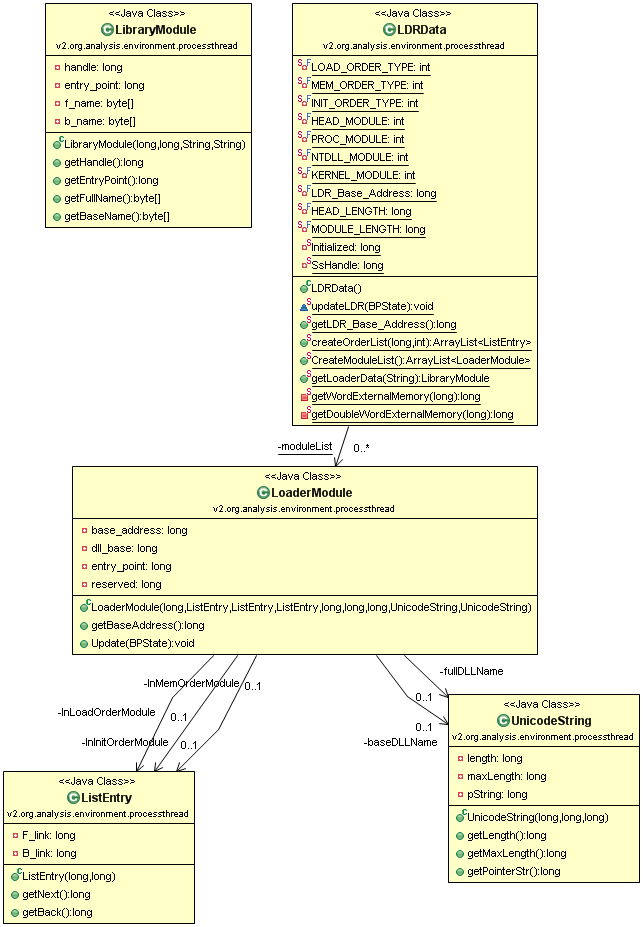
\includegraphics[width=0.5\textwidth]{ldr}
\caption{Cấu trúc của LDR Data}
\label{fig:LDRArchi}
\end{figure}
}
\item{\textbf{Trap Flag}: để có thể xử lý kỹ thuật SEH sử dụng Trap Flag của Packer thì hệ thống BE-PUM được hỗ trợ một lớp để có thể lưu trữ những giá trị địa chỉ của hàm xử lý ngoại lệ, ngoài ra hệ thống BE-PUM còn được hỗ trợ thêm 8 thanh ghi gồm: DRO, DR1, DR2, DR3, DR4, DR5, DR6, DR7. Hình \ref {fig:SEHHandlerArchi} mô tả lớp dùng để xử lý SEH khi có sự thay đổi giá trị trong 8 thanh ghi debug.
\begin{figure}
\centering
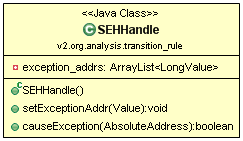
\includegraphics[width=0.5\textwidth]{seh}
\caption{Cấu trúc của SEH Handler}
\label{fig:SEHHandlerArchi}
\end{figure}
}
\item{\textbf{Virtual Memory Block}: để có thể xử lý kỹ thuật Stolen Bytes trong packer. Một lớp được hiện thực để quản lý nếu quá trình mở gói được thực hiện trên vùng nhớ ảo. Hình \ref {fig:VirtualMemArchi} mô tả lớp quản lý vùng nhớ ảo được hiện thực trong hệ thống BE-PUM.
\begin{figure}
\centering
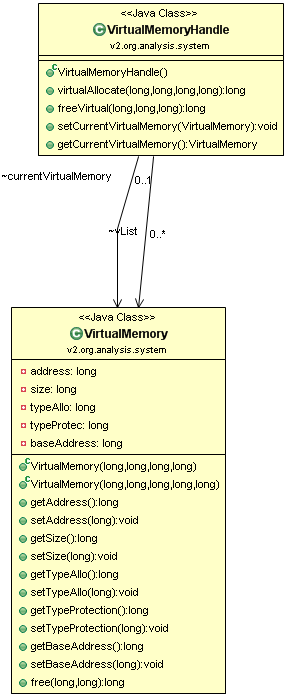
\includegraphics[width=0.5\textwidth]{virtual_mem}
\caption{Cấu trúc của một Virtual Memory Handler}
\label{fig:VirtualMemArchi}
\end{figure}
}
\end{itemize}

\section{Thiết kế giải thuật nhận dạng Packer thông qua chữ ký}

\hspace{0.5cm}Phương pháp nhận dạng thông qua chữ ký được sử dụng trong các phần mềm như PEID, CFF Explorer. Ưu điểm của phương pháp nhận dạng chữ ký là quá trình nhận dạng không tốn quá nhiều thời gian, công sức. Chữ ký là một chuỗi byte có duy nhất tương ứng với mỗi packer, do đó nhược điểm lớn nhất là những chữ ký này luôn được packer thay đổi sau mỗi lần nâng cấp phiên bản nhằm ẩn thân trước các công cụ nhận dạng.\\

\hspace{0.5cm}Giải thuật nhận dạng chữ ký của packer sẽ bao gồm công việc thu thập những chữ ký này và xử lý dữ liệu thô. Dữ liệu sẽ được lưu trữ dưới dạng dữ liệu JSON qua đó cho phép BE-PUM dễ dàng sửa đổi và thêm mới các chữ ký này.

\begin{code}
\begin{lstlisting}[captionpos=b,caption={Cấu trúc lưu trữ của một chữ ký},frame=single]
{
  "PACKER_NAME"    : name
  "VERSION"        : version
  "IS_ENTRY_POINT" : yes/no
  "SIGNATURE"      : bytes array
}
\end{lstlisting}
\end{code}

\hspace{0.5cm}BE-PUM sẽ chuyển đổi dữ liệu JSON lưu trữ chữ ký này thành dữ liệu lưu trữ dưới dạng mảng các byte. Thuộc tính "IS\_ENTRY\_POINT" sẽ xác định nếu quá trình nhận dạng chữ ký này sẽ bắt đầu kiểm tra từ header hay từ vị trí entry point của tập tin. Nếu giá trị này là TRUE, quá trình kiểm tra sẽ bắt đầu từ vị trí entry point, và ngược lại nếu giá trị này là FALSE, quá trình kiểm tra sẽ bắt đầu từ vị trí header đến vị trí entry point. Vì packer có thể nâng cấp những phiên bản mới nhằm mục đích thay đổi chữ ký này, do đó BE-PUM cũng sẽ lưu trữ lại phiên bản của packer thông qua thuộc tính "VERSION".\\ 

\hspace{0.5cm}Quá trình kiểm tra sẽ so trùng từng byte của tập tin thực thi với mảng các byte của chữ ký, bước đầu sẽ tiến hành so trùng ít nhất 2 byte đầu của chữ ký và tập tin. Nếu trong trường hợp, 2 giá trị này trùng với 2 giá trị của chữ ký thì một quá trình kiểm tra so trùng toàn bộ chữ ký được thực hiện. Nếu trùng với chữ ký của packer thì BE-PUM sẽ trả về tên của packer và phiên bản của packer. Ngược lại, quá trình sẽ trả về giá trị rỗng. Đoạn mã giả \ref {lst:SignatureAlgo} mô tả về giải thuật nhận dạng packer thông qua phương pháp nhận dạng chữ ký.

\begin{code}
\begin{lstlisting}[captionpos=b,caption={Giải thuật nhận dạng packer thông qua chữ ký},label={lst:SignatureAlgo},frame=single,language=Python]
data = ReadFile(file)
for signature in signature_data:
  begin_tracing = 0
  end_tracing = 0
  pivot = 0
  entry_point = GetEntryPoint(file)
  for byte in data:
    if byte == entry_point:
      pivot = byte.index
      break
  if signature.WillTraceFromEntryPoint():
    begin_tracing = pivot
    end_tracing = pivot + signature.data.length() + 1
  else
    begin_tracing = 0
    end_tracing = pivot
	
  isTrace = true
  for i in range(begin_tracing, end_tracing) and isTrace:
    if signature.data[i] == data[i] 
      and signature.data[i+1] == data[i+1]:
      for j in range(0, data.length()):
        if i + j < data.length():
          if not signature.data[j] == data[i+j]:
            break
          else if j == data.length() - 1:
            isTrace = false
        else
          return false
    else if begin_tracing != 0 or i == end_tracing - 2 
      return false
return true
\end{lstlisting}
\end{code}

\section{Kết hợp hệ thống BE-PUM và NuSMV}

\hspace{0.5cm}Chính vì những nhược điểm của quá trình nhận dạng packer thông qua chữ ký, mà việc nhận dạng packer bằng phương pháp nhận dạng thông qua ngữ nghĩa được áp dụng, cụ thể là quá trình kết hợp giữa hệ thống BE-PUM và công cụ kiểm tra mô hình NuSMV. Công việc được thực hiện bao gồm việc xây dựng mô hình NuSMV và mô tả những kỹ thuật của packer thông qua biểu thức CTL.

\subsection{Thiết kế và xây dựng NuSMV Model}
\hspace{0.5cm}Việc thiết kế và xây dựng một mô hình NuSMV để có thể kiểm tra với công cụ NuSMV bao gồm 2 giai đoạn chính: thứ nhất là chuyển đổi mô hình của BE-PUM thành dữ liệu JSON để có thể dễ lưu trữ và sử dụng hơn, và thứ hai là quá trình chuyển đổi dữ liệu JSON thành mô hình NuSMV.

\subsubsection{Chuyển đổi mô hình BE-PUM và dữ liệu JSON}

\hspace{0.5cm}Quá trình chuyển đổi mô hình của hệ thống BE-PUM sang dữ liệu JSON để đảm bảo không tốn quá nhiều thời gian để hiểu được cấu trúc của một CFG của BE-PUM, cũng như có thể được sử dụng như đầu vào cho bất kì một công cụ kiểm tra mô hình, không xử lý quá nhiều để có thể đọc vào dữ liệu JSON này cũng là một điểm mạnh.\\

\hspace{0.5cm}Một dữ liệu JSON mô tả cho mô hình của BE-PUM sẽ bao gồm một tập các node và edge được biểu diễn như mảng JSON, trong đó mỗi node và edge là những đối tượng JSON được định nghĩa là địa chỉ của câu lệnh tại node đó và nội dung của câu lệnh đó, mỗi edge được định nghĩa bởi source và destination, với source và destination là địa chỉ của các node.\\

\hspace{0.5cm}Để chuyển đổi hệ thống BE-PUM sang dữ liệu JSON, lớp CFGUtil được xây dựng và tích hợp trong hệ thống BE-PUM. Hình \ref {fig:CFGUtilArchi} mô tả lớp với vai trò chuyển đổi giữa mô hình CFG của BE-PUM sang dữ liệu JSON.

\begin{figure}
\centering
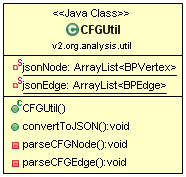
\includegraphics[width=0.5\textwidth]{cfg_to_json}
\caption{Lớp chuyển đổi CFG của BE-PUM sang dữ liệu JSON}
\label{fig:CFGUtilArchi}
\end{figure}

\hspace{0.5cm}Dữ liệu JSON \ref {lst:CFGJSON} minh hoạ về dữ liệu JSON được chuyển đổi từ mô hình CFG \ref {fig:JSONCFG} của BE-PUM.

\begin{code}
\begin{lstlisting}[captionpos=b,caption={Dữ liệu JSON được chuyển đổi từ CFG của BE-PUM},label={lst:CFGJSON},frame=single]
{
  "model":
  {
    "nodes":
    [
      {
        "loc"	: "0x00401000",
        "inst"	: "inc %eax"
      },
      {
        "loc"	: "0x00401001",
        "inst"	: "jne 0x00401000"
      },
      {
        "loc"	: "0x00401006",
        "inst"	: "pushl %eax"
      }
    ],
    "edges":
    [
      {
        "src"	: "0x00401000",
        "dest"	: "0x00401001"
      },
	  {
        "src"	: "0x00401001",
        "dest"	: "0x00401006"
      },
      {
        "src"	: "0x00401001",
        "dest"	: "0x00401000"
      }
    ]
  }
}

\end{lstlisting}
\end{code}

\begin{figure}
\centering
\begin{tikzpicture}[shorten >=1pt,node distance=2cm,on grid,auto] 
   	\node[cfgstate,align=center](s_1){0x00401000\\\ inc \%eax}; 
   	\node[cfgstate,align=center](s_2)[below of=s_1]{0x00401001\\\ jne 0x00401000};
   	\node[cfgstate,align=center](s_3)[below of=s_2]{0x00401006\\\ pushl \%eax};
    \path[-{>[scale=2,length=3,width=3]}] 
    (s_1) edge node {} (s_2)
  	(s_2.east) edge [bend right=60] node {} (s_1.east)
    (s_2) edge node {} (s_3);	  
\end{tikzpicture}
\caption{Ví dụ về mô hình CFG của BE-PUM được chuyển đổi JSON}
\label{fig:JSONCFG}
\end{figure}

\subsection{Chuyển đổi dữ liệu JSON và mô hình NuSMV}

\hspace{0.5cm}Trong thực tế, một packer có rất nhiều phiên bản và sử dụng nhiều biến thể của kỹ thuật. Packer có thể thay đổi câu lệnh đó một cách khác đi nhưng không thay đổi kết quả của kỹ thuật đó mang lại. Hình \ref {fig:SEHNuSMV} mô tả một ví dụ về sử dụng kỹ thuật SEH tiêu chuẩn trong một packer và biến thể của SEH, theo đó thay bằng việc PUSH một giá trị constant vào stack, thì packer sẽ thiết lập giá trị này cho thanh ghi EAX và push trực tiếp thanh ghi EAX vào stack.

\begin{figure}
\centering
\begin{tabular}[c]{cc}
	\subfloat[SEH tiêu chuẩn]
	{
		\label{fig:StandardSEH}
		\begin{tikzpicture}[shorten >=1pt,node distance=2cm,on grid,auto] 
   			\node[cfgstate](s_1){pushl 0x00401020}; 
   			\node[cfgstate](s_2)[below of=s_1]{pushl \%fs:[0]};
   			\node[cfgstate](s_3)[below of=s_2]{movl \%fs:[0],\%esp};
    		\path[-{>[scale=2,length=3,width=3]}] 
    			(s_1) edge node {} (s_2)
  				(s_2) edge node {} (s_3);
		\end{tikzpicture}
    }
    &
	\subfloat[Biến thể của SEH]
	{
		\label{fig:VariantSEH}
        \begin{tikzpicture}[shorten >=1pt,node distance=2cm,on grid,auto] 
        	\node[cfgstate](s_0){movl \%eax, 0x00401020}; 
   			\node[cfgstate](s_1)[below of=s_0]{pushl eax}; 
   			\node[cfgstate](s_2)[below of=s_1]{pushl \%fs:[0]};
   			\node[cfgstate](s_3)[below of=s_2]{movl \%fs:[0],\%esp};
    		\path[-{>[scale=2,length=3,width=3]}] 
    			(s_0) edge node {} (s_1)
    			(s_1) edge node {} (s_2)
  				(s_2) edge node {} (s_3);
		\end{tikzpicture}
	}
\end{tabular}
\caption{Sự đa dạng trong kỹ thuật SEH}
\label{fig:SEHNuSMV}
\end{figure}

\hspace{0.5cm}Chính vì sự đa dạng đó, mà quá trình chuyển đổi dữ liệu JSON sang mô hình NuSMV không chỉ đơn giản là việc chuyển đổi toàn bộ giá trị ký hiệu vào trong mô hình vì rất khó để có thể mô tả hết tất cả các biến thể kỹ thuật. Vì thế, trước khi xây dựng mô hình NuSMV, quá trình phân loại các register, segment register, giá trị immediate và lệnh gọi API được thực hiện bằng việc:

\begin{itemize}
\item{Phân loại câu lệnh theo mnemonic của câu lệnh: câu lệnh sẽ được phân loại thuộc X86ArithmeticInstruction, X86CallInstruction, X86CondJumpInstruction, X86JmpInstruction, X86MoveInstruction, X86RetInstruction.}
\item{Phân loại các register: 16 thanh ghi sẽ được phân loại thuộc X86Register.}
\item{Phân loại các segment register: 4 segment register sẽ được phân loại thuộc X86SegmentRegister.}
\item{Phân loại các giá trị immediate: các giá trị constant được biểu diễn dưới dạng hexa sẽ được phân loại thuộc X86ImmediateValue.}
\item{Phân loại các lệnh gọi API: các lệnh gọi API sẽ được phân loại thuộc X86APICalling.}
\end{itemize}

\hspace{0.5cm}Hình \ref {fig:SMVModelChecking} mô tả các lớp của hệ thống chuyển đổi dữ liệu JSON sang mô hình NuSMV.

\begin{figure}
\centering
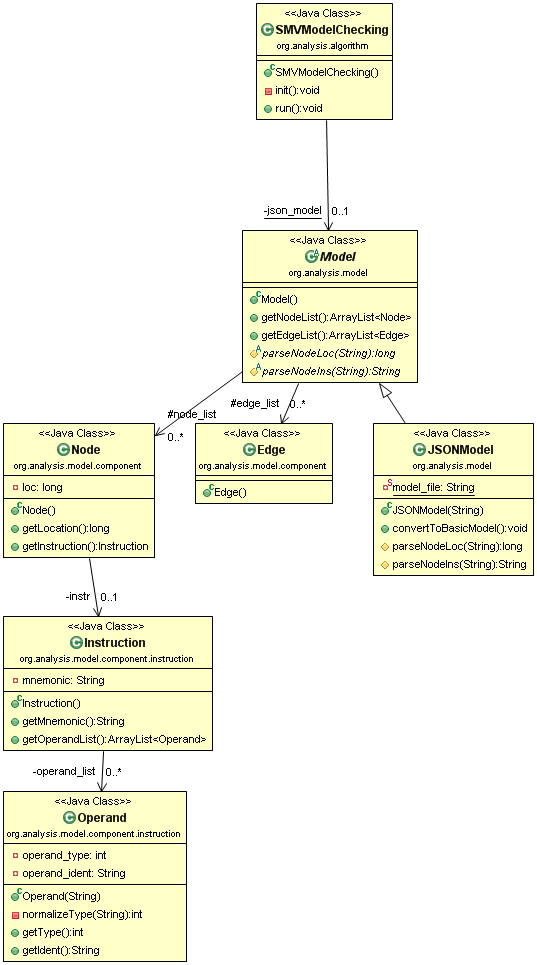
\includegraphics[width=0.7\textwidth]{smv_model_checking}
\caption{Kiểm tra mô hình kết hợp NuSMV}
\label{fig:SMVModelChecking}
\end{figure}

